%****************************************************************
% Chapter X
%****************************************************************
\label{chapter-technology}
\chapter{Technology}

In this chapter, details of the related technologies are presented. They are Android smartphone, a low-cost way to experience immersive virtual reality environment; OpenGL ES in Android; KML for geographic visualization; Golang RESTful web server for managing data in the back-end.

%****************************************************************
\section{Virtual Reality Device}

There are following reasons for using Android smartphone as the virtual reality device. The intention is to identify immersive virtual reality device that not only low-cost but also a standard, customer-friendly device. That is the smartphone, and it had an incredibly fast growth trend in the last few years and a good promising market prospect \ref{fig:smartphone-shipments-forecast}. After all, it contains all the necessary sensors and positioning systems to measure motion and accurately track device movements - Six degrees of freedom (DOF) - position coordinates (x, y and z offsets) and orientation (yaw, pitch and roll angles). Additionally, 15\$ Google Cardboard kit turns Android or iOS smartphone to immersive virtual reality device. According to International Data Corporation (IDC), Android dominated the smartphone market with a share of 87.6\% in the worldwide \ref{fig:smartphone-os-market-share}. Moreover, there is an existing Google VR SDK \cite{google.vr-sdk.2016} for Android supports.

\begin{figure}[H]
\caption[Global Smartphone Shipments Forecase]{Global Smartphone Shipments Forecase \cite{tony.global-smartphone-market.2015}}
\label{fig:smartphone-shipments-forecast}
\centering
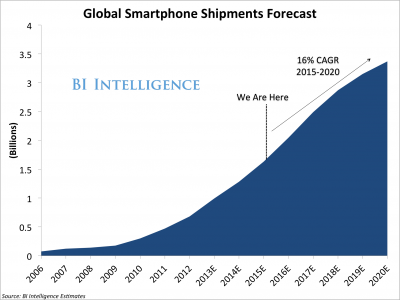
\includegraphics[width=0.7\textwidth, keepaspectratio]{Figures/smartphone-shipments-forecast.png}
\decoRule
\end{figure}

\begin{figure}[H]
\caption[Smartphone OS Market Share]{Smartphone OS Market Share \cite{idc.smartphone-os-market-share.2016}}
\label{fig:smartphone-os-market-share}
\centering
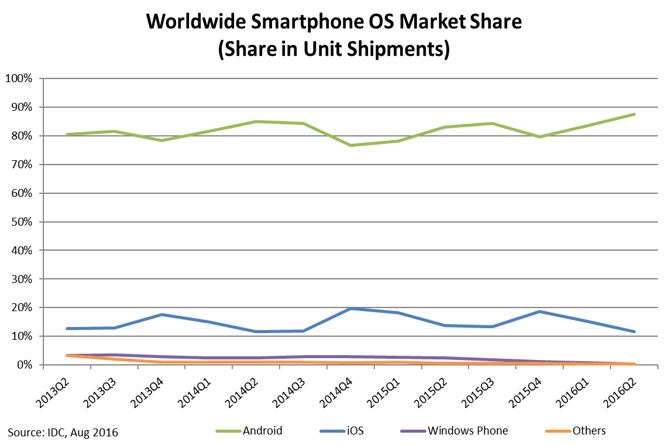
\includegraphics[width=0.7\textwidth, keepaspectratio]{Figures/smartphone-os-market-share.png}
\decoRule
\end{figure}

%****************************************************************
\section{OpenGL ES}

Android includes support for high-performance 2D and 3D graphics with the Open Graphics Library, specifically, the OpenGL ES API \cite{google.opengles.2016}. OpenGL ES is a branch of the OpenGL specification intended for embedded devices. The Google VR SDK requires the device has a minimum OpenGL ES 2.0 support. Table \ref{tab:opengles-spec-android} shows a version list of OpenGL ES API that Android supported.

\begin{table}[H]
\caption{OpenGL ES API specification supported by Android}
\label{tab:opengles-spec-android}
\centering
\begin{tabular}{l l l}
\toprule
\tabhead{OpenGL ES Version} & \tabhead{Android Version}\\
\midrule
OpenGL ES 1.0 & Android 1.0 and higher\\
OpenGL ES 1.1 & Android 1.0 and higher\\
OpenGL ES 2.0 & Android 2.2 (API level 8) and higher\\
OpenGL ES 3.0 & Android 4.3 (API level 18) and higher\\
OpenGL ES 3.1 & Android 5.0 (API level 21) and higher\\
OpenGL ES 3.2 (September 2016) & Android 7.0 (API level 24) and higher\\
\bottomrule
\end{tabular}
\end{table}

%****************************************************************
\section{Geographic Visualization Markup Language}

I was looking for a simple markup language for geographic data visualization. It should be not only able to represent a geographic data in the virtual reality, but also be beneficial to publish and consume data in interoperable formats without the needs of technical assistance. 

The Keyhole Markup Language (KML) can be combined with other supporting files such as imagery in a zip archive, producing a KMZ file. KML offers features for expressing geographic annotation and visualization. The annotations of KML features are not designed as machine-readable XML, but a human readable plain text or simple HTML. The \code{Networklink} facility in KML contributes to a real-time data which is important in the environmental sciences. It allows all or part of the dataset to be automatically refreshed by the URL, to ensure the user always sees the latest information.

More importantly than the satisfaction of needs in the application, it supported by many virtual globes and other GIS systems. Therefore the KML already becoming a de facto standard \cite{blower.sharing-visualizing.2007} that can be manipulated in other softwares if required. 

\begin{figure}[H]
\caption[KML schema]{KML schema \cite{google.kml.2016}}
\label{fig:kml-schema}
\centering
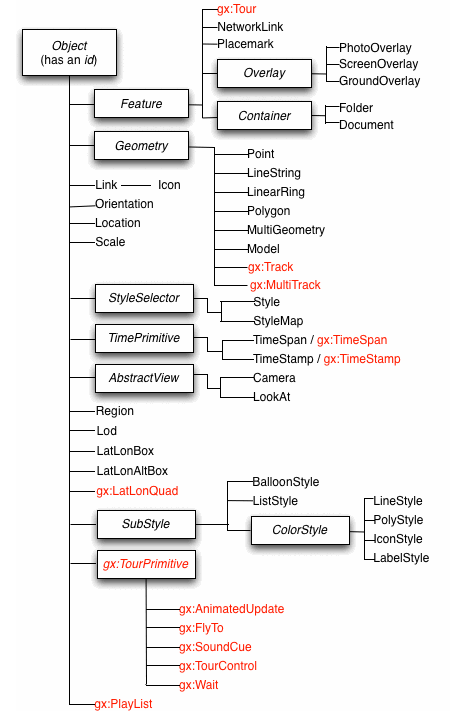
\includegraphics[height=0.7\textheight, keepaspectratio]{Figures/kml-schema.png}
\decoRule
\end{figure}

%****************************************************************
\section{Network}
\label{section:network}

Real-time data are very important in the environmental sciences \cite{blower.sharing-visualizing.2007}. One of the key strengths of virtual reality applications are not only easy-to-use, and intuitive nature, but also the ability to efficiently incorporate new data.  Therefore, a web server is needed. A RESTful web server to support communication with the client, and a remote file server to synchronize data are included in the application.

Go (often referred to as golang \cite{google.golang.2016}) is an open source programming language, and it is compiled, concurrent, garbage-collected, statically typed language developed at Google in late 2007. It was conceived as an answer to some of the problems they were seeing and developing software infrastructure \cite{google.talk-golang.2012}. Surprisingly, the rise of Go was growing so fast that each month the contributors outside Go team itself are already more than the contributors inside the Go team. Additionally, Golang is well suited for developing RESTful API’s. Its net/http standard library provides a set of key methods for interacting via the HTTP protocol. For the above reasons, the Golang is selected in this paper for developing the server. 

On the client side (Android platform), Volley is being used for transmitting network data (Volley is an open sourced HTTP library that makes networking for Android apps easier and most importantly, faster \cite{google.volley.2016}). Furthermore, Jsoup (Java HTML Parser \cite{joup.2016}) is being introduced for analyzing HTML format response.

%****************************************************************
